\documentclass[aip]{revtex4-1}

\setlength{\oddsidemargin}{0in}  %left margin position, reference is one inch
\setlength{\textwidth}{6.5in}    %width of text=8.5-1in-1in for margin
\setlength{\topmargin}{-0.5in}    %reference is at 1.5in, -.5in gives a start of about 1in from top
\setlength{\textheight}{9in}     %length of text=11in-1in-1in (top and bot. marg.) 

\usepackage{amsmath,amssymb}
\usepackage{graphicx}% Include figure files
\usepackage{color}% Include colors for document elements
\usepackage{dcolumn}% Align table columns on decimal point
\usepackage{bm}% bold math

\definecolor{background-color}{gray}{0.98}
\graphicspath{{data/}{images/}}

  \makeatletter
  \renewcommand\@biblabel[1]{#1.}
  \makeatother

\bibliographystyle{apsrev}

\begin{document}

\renewcommand{\thetable}{S-\Roman{table}}
\renewcommand{\thefigure}{S-\Roman{figure}}

\title{Atomic pseudo-potentials for reproducing the valence electron behaviour of sp$^2$ carbon atoms: Supplementary Material}
\author{Alexander Punter}
\author{Paola Nava}
\author{Yannick Carissan}
\affiliation{Aix Marseille Univ, CNRS, Centrale Marseille, iSm2, Marseille, France}

\maketitle

\tableofcontents

\section*{Details on the extraction process}
\subsection*{CH\(_{3}\), with \(s\) potentials}

We aim first to reproduce the values for the CH\(^{\bullet}_{3}\) radical as given in Table \ref{table:ch3_s_potentials}. 
This reference CH\(^{\bullet}_{3}\) is created and has its geometry optimised under Hartree-Fock (HF/def-SV(P)). The reference geometry gives a C - H distance of 2.0466 a.u., and so we pick \(d = 2.0\) a.u. as a starting guess for the planar distance from the pseudo-carbon, \(d\), of our pseudo-potentials. The pseudo-system is then set up, erasing the hydrogen atoms, setting the carbon charge \(Z_{nucleus} = 1\) and applying \(s\) pseudo-potentials, as well as selecting the correct orbital for the remaining electron. Table \ref{table:ch3_s_potentials} displays some of our results. Promisingly, we are able to produce many sets of potentials that give the correct energy.

\begin{table}[ht]
\caption{Coefficients and exponents for \(s\)-only pseudo-potentials for CH\(^{\bullet}_{3}\), optimised to give 
the all-electron HOMO reference energy of  -10.537~eV (HF) and -6.726~eV (PBE0). 
\(d = 0.5\) a.u., as defined in Figure 1.}
\label{table:ch3_s_potentials}
\begin{tabular}{c c c}
\hline\hline
 & Coefficient & Exponent \\ 
\hline
HF & -2.594 & 1.0 \\
 & -4.788 & 5.0 \\
 & -7.524 & 10.0 \\
\hline
PBE0 & -2.605 & 1.0 \\
 & -4.873 & 5.0 \\
 & -7.678 & 10.0 \\
\hline\hline
\end{tabular}
\end{table}

\subsection*{Ethene, with \(s\) and \(p\) potentials}

Next, we take some of these potentials to create a pseudo-ethene system, with the results shown in Table \ref{table:ethene_s_pseudo}. All potentials tested with \(d = 2.0\) a.u. gave results several orders of magnitude away from the reference value. From Figure \ref{fig:long_r_ethene} we may see the reason. One of the potential sets from each carbon is closer to the neighbouring carbon than the neighbour's own potential sets, thus both pseudo-carbons are affected by potentials which do not belong to them. At the shorter range \(d = 0.5\) a.u., the HOMO energy is of the right magnitude, though with errors of \(~ 30\%\). Attempts to eliminate this error lead us to the additional use of the \(p_{z}\) potential \textit{alongside} the \(s\) potentials.

\begin{table}[ht]
\caption{HOMO energies ($\pi$, eV) for ethene and pseudo-ethene. The pseudo-potentials used in the pseudo-ethene are taken from optimised values for 
pseudo-CH\(^{\bullet}_{3}\) with only \(s\) potentials and an exponent of 10.0. $d$ (a.u.) as defined 
in Figure 1.}
\label{table:ethene_s_pseudo}
\begin{tabular}{c c c c}
\hline\hline
& $d$ & \(s\) coefficient & \( \pi \)  \\
\hline
HF$^a$   &     &        & -10.363 \\
PBE0$^a$ &     &        & -6.632 \\
HF       & 2.0 & -7.521 & -9597.0 \\
HF       & 0.5 & -7.521  & -7.905 \\
PBE0     & 0.5 &-7.678  & -8.447 \\
\hline\hline
\multicolumn{4}{l}{$^a$ All-electron reference values.}\\
\end{tabular}
\end{table}

\begin{figure}
\begin{center}
\fbox{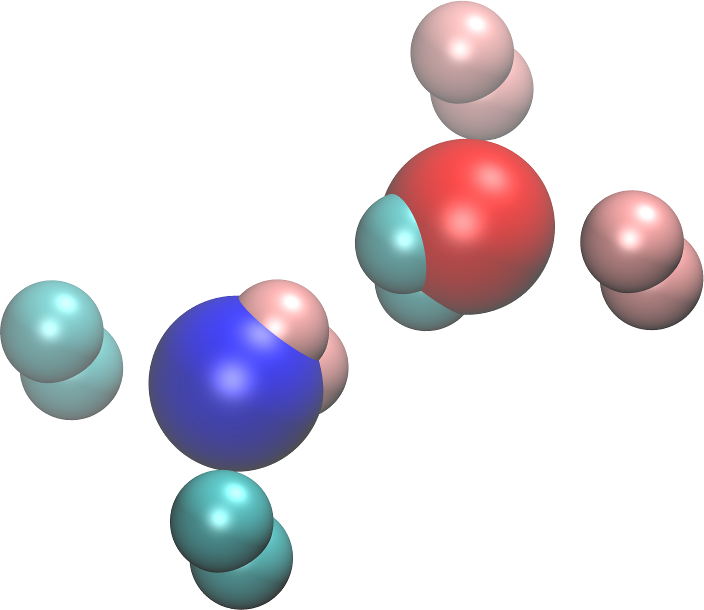
\includegraphics[width=0.45\textwidth]{hires_long_r_crop.png}}%
\fbox{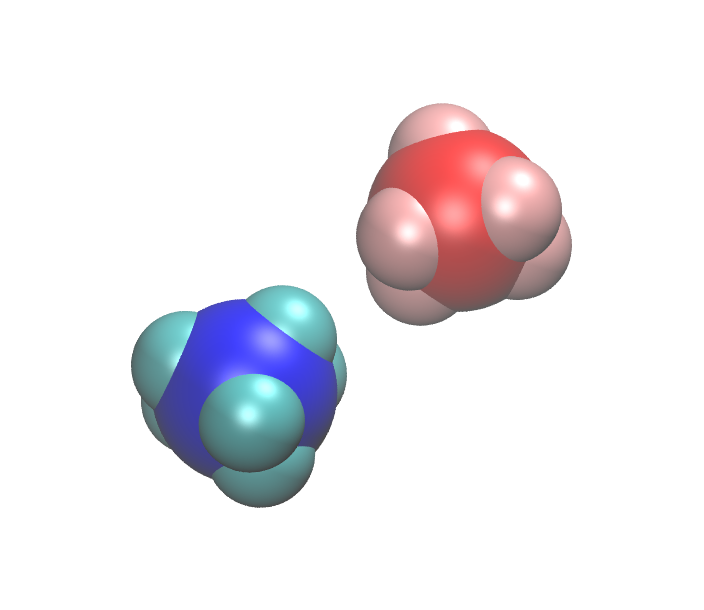
\includegraphics[width=0.45\textwidth]{hires_short_r_crop.png}}
\end{center}
\caption{Diagrams of pseudo-ethene with \(d =\) 2.0 a.u. (left), and \(d = 0.5\) a.u. (right). The first pseudo-carbon is displayed in blue, with its \(s\) pseudo-potentials in cyan, and the second pseudo-carbon is in red, with its potentials in pink.}
\label{fig:long_r_ethene}
\end{figure}

The next step adds a \(p\) potential centred on the pseudo-carbon, with Table \ref{table:p_potentials} displaying the results. As before, \(d = 0.5\) a.u.. The \(p_{z}\) potential is selected using the procedure described in Section II B, with the exponent chosen to give the maximum possible overlap with the \(p_{z}\) orbital, and the matching \(Z_{eff}\) coefficient calculated from the exponent and overlap. The \(s\) potentials are then optimised once more to give the correct HOMO energy for CH\(^{\bullet}_{3}\). We again take these potentials to create a pseudo-ethene molecule, with the results shown in Table \ref{table:p_potentials}. We can see that these potentials seem to transfer more effectively from the CH\(^{\bullet}_{3}\) system to the ethene, suggesting therefore that whilst the \(s\) potentials can affect both the \(p_{z}\) and \(\pi\) orbitals, they 
cannot alone describe the relationship between them.

\begin{table}[ht]
\caption{\(\pi\) orbital energy values (eV) for pseudo-ethene, using \(s\) and \(p\) pseudo-potentials.
The pseudo-potentials are taken from a pseudo-CH\(^{\bullet}_{3}\) system optimised to give the correct all-electron HOMO energy.}
\label{table:p_potentials}
\begin{tabular}{c c c c}
\hline\hline
& \(p\) coefficient & \(p\) exponent \\
\hline
\(p_{z}\) potential & -3.267 & 0.295 \\
\hline
Calculation Type & \(s\) coefficient & \(s\) exponent & \(\pi\) \\
\hline
HF & 2.772 & 1.0 & -13.654 \\
 & 6.173 & 5.0 & -14.011 \\
 & 10.381 & 10.0 & -14.061 \\
\hline
PBE0 & 3.483 & 1.0 & -10.325 \\
 & 9.801 & 5.0 & -10.409 \\
 & 18.351 & 10.0 & -12.543 \\
\hline\hline
\end{tabular}
\end{table}

Having successfully created a pseudo-ethene with the correct HOMO, we attempt to have the pseudo-system replicate other properties of the real system:
the singlet-triplet excitation energy ($\Delta_{ST}$) in the SCF framework (energy difference between the triplet and the singlet mono-reference
calculations), the ionisation energy (IE) and the energy of the HOMO orbital ($\varepsilon_{HOMO}$). Reference values for the singlet-triplet \(\pi-\pi^{*}\) excitation and first ionisation energies of ethene are given in Table III. Testing the relevant energies for the optimised pseudo-systems above, we found that the early results were not promising. However, after we abandon the notion of sticking strictly to a \(p_{z}\) potential exponent that gives the maximum overlap with the real orbital, we discover there is a "sweet spot" of potential coefficients and exponents around which the correct values begin to emerge. Tables II and III show our optimal result, chosen to give HOMO, ($\Delta_{ST}$) and ionisation energies closest to the reference values. 

\subsection*{Optimisation}

In earlier calculations with only \(s\) potentials, optimisation was performed by choosing a range of exponent values and attempting to optimise the coefficient at each to produce the HOMO reference energy. Once the \(p_{z}\) potential was added, the \(s\) potentials were optimised afterward. 

Once we started to look at excitation and ionisation energies however, optimisation became more complicated. Optimisations were at first performed of the $s$ and $p$ potentials to reach the HOMO energy of ethene as before. With the different potential variables available, we produced a range of optimised potential sets. The best set of these potentials was then chosen and the values altered by hand in order to match as closely as possible three separate reference values: the singlet HOMO energy, the singlet-triplet \(\pi-\pi^{*}\) excitation energy, and the cation-singlet energy. All optimisations used the Brent method in SciPy's optimisation library, with a tolerance of \(1.48*10^{-08}\), and used standard Hartree-Fock calculations.

\section*{Method Comparison: Frozen Orbitals}

We computed the ionisation potentials of the small alkenes at the Hartree-Fock level in the frozen approximation in order to
quantify the effect of neglecting the reorganisation of the $\sigma$ molecular orbitals in the cation. To do that, we froze
the $\sigma$ doubly-occupied orbitals in the cations, as they were obtained in the calculations for the neutral system, Table~\ref{tab:froz_comp}
and Figure~\ref{fig:froz_comp}.
Those calculations were performed with the MOLCAS program package.

\begin{table} 
\caption{All-electron Hartree-Fock ionisation energies computed for short alkene chains. 
The frozen values are obtained by freezing the doubly-occupied $\sigma$ molecular orbitals in the cation
as they obtained in the neutral system.}
\label{tab:froz_comp}
\begin{tabular}{lrrrr}
\hline
\multicolumn{5}{c}{Ionisation Energies (IE) in eV} \\
              & IE Reference  &  IE Frozen& Error & \% Error \\
\hline
$\text{C}_{2}\text{H}_{4}$  & 10.06  &   9.11 &  0.95  & 10.38 \\
$\text{C}_{4}\text{H}_{6}$  & 8.82   &   8.09 &  0.73  & 9.04 \\
$\text{C}_{6}\text{H}_{8}$  & 8.10   &   7.38 &  0.72  & 9.70 \\
$\text{C}_{8}\text{H}_{10}$ & 7.65   &   6.96 &  0.69  & 9.86 \\
$\text{C}_{10}\text{H}_{12}$& 7.35   &   6.67 &  0.68  & 10.21 \\
$\text{C}_{12}\text{H}_{14}$& 7.15   &   6.47 &  0.67  & 10.40 \\
\hline
Average &&&                        0.74  & 9.93 \\
\hline
\end{tabular}
\end{table} 

\begin{figure}
\begin{center}
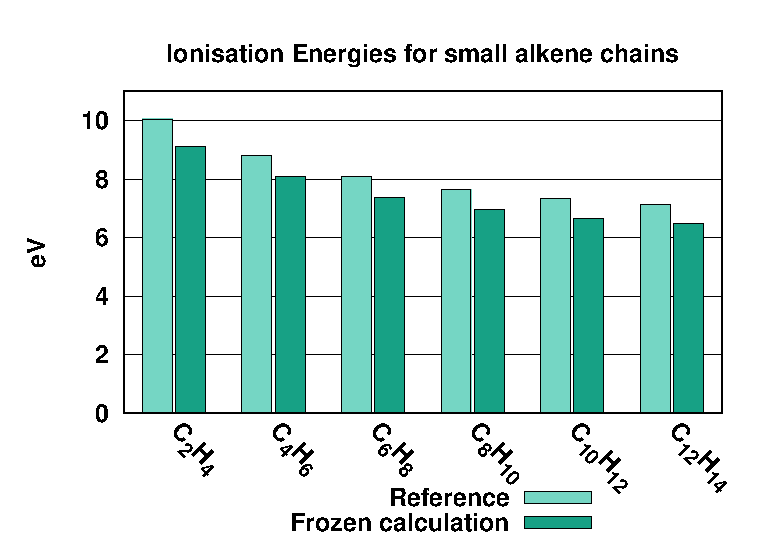
\includegraphics[width=8cm]{froz_comp}
\end{center}
\caption{Computed ionisation energies for small alkene-chains. Reference calculations are all-electron Hartree-Fock calculations, frozen calculation 
are all-electron calculation where the $\sigma$ orbitals were frozen in the cation as they were obtained in the neutral system.}
\label{fig:froz_comp}
\end{figure}

%\section*{Method Comparison: TDDFT and CASPT2}
%
%\begin{figure}
%\begin{center}
%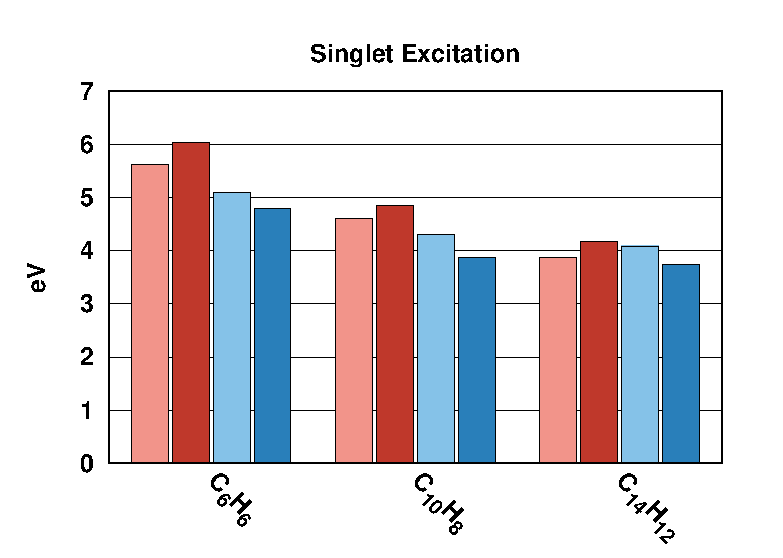
\includegraphics[width=8cm]{methodcomp_s_excitations}
%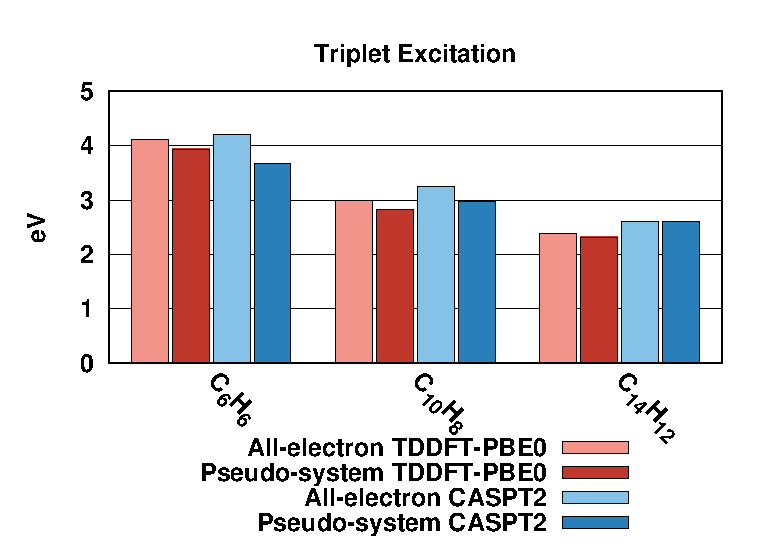
\includegraphics[width=8cm]{methodcomp_t_excitations}
%\end{center}
%\caption{Comparison of all-electron and pseudo-molecules for TDDFT-PBE0 and CASPT2 methods across ethylene, benzene, naphthalene and anthracene systems.}
%\label{fig:method_comp}
%\end{figure}

\section*{Comparison with our previous study}
\begin{figure}
\begin{center}
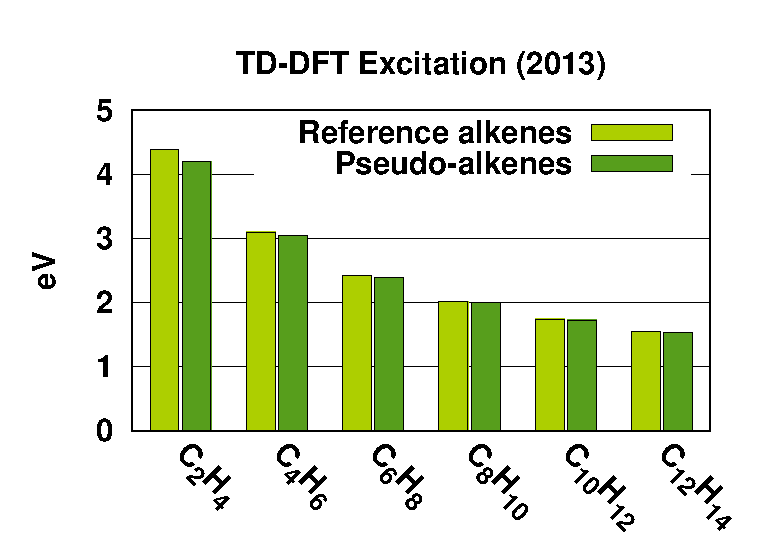
\includegraphics[width=8cm]{short_pbe0_tddft_2013}
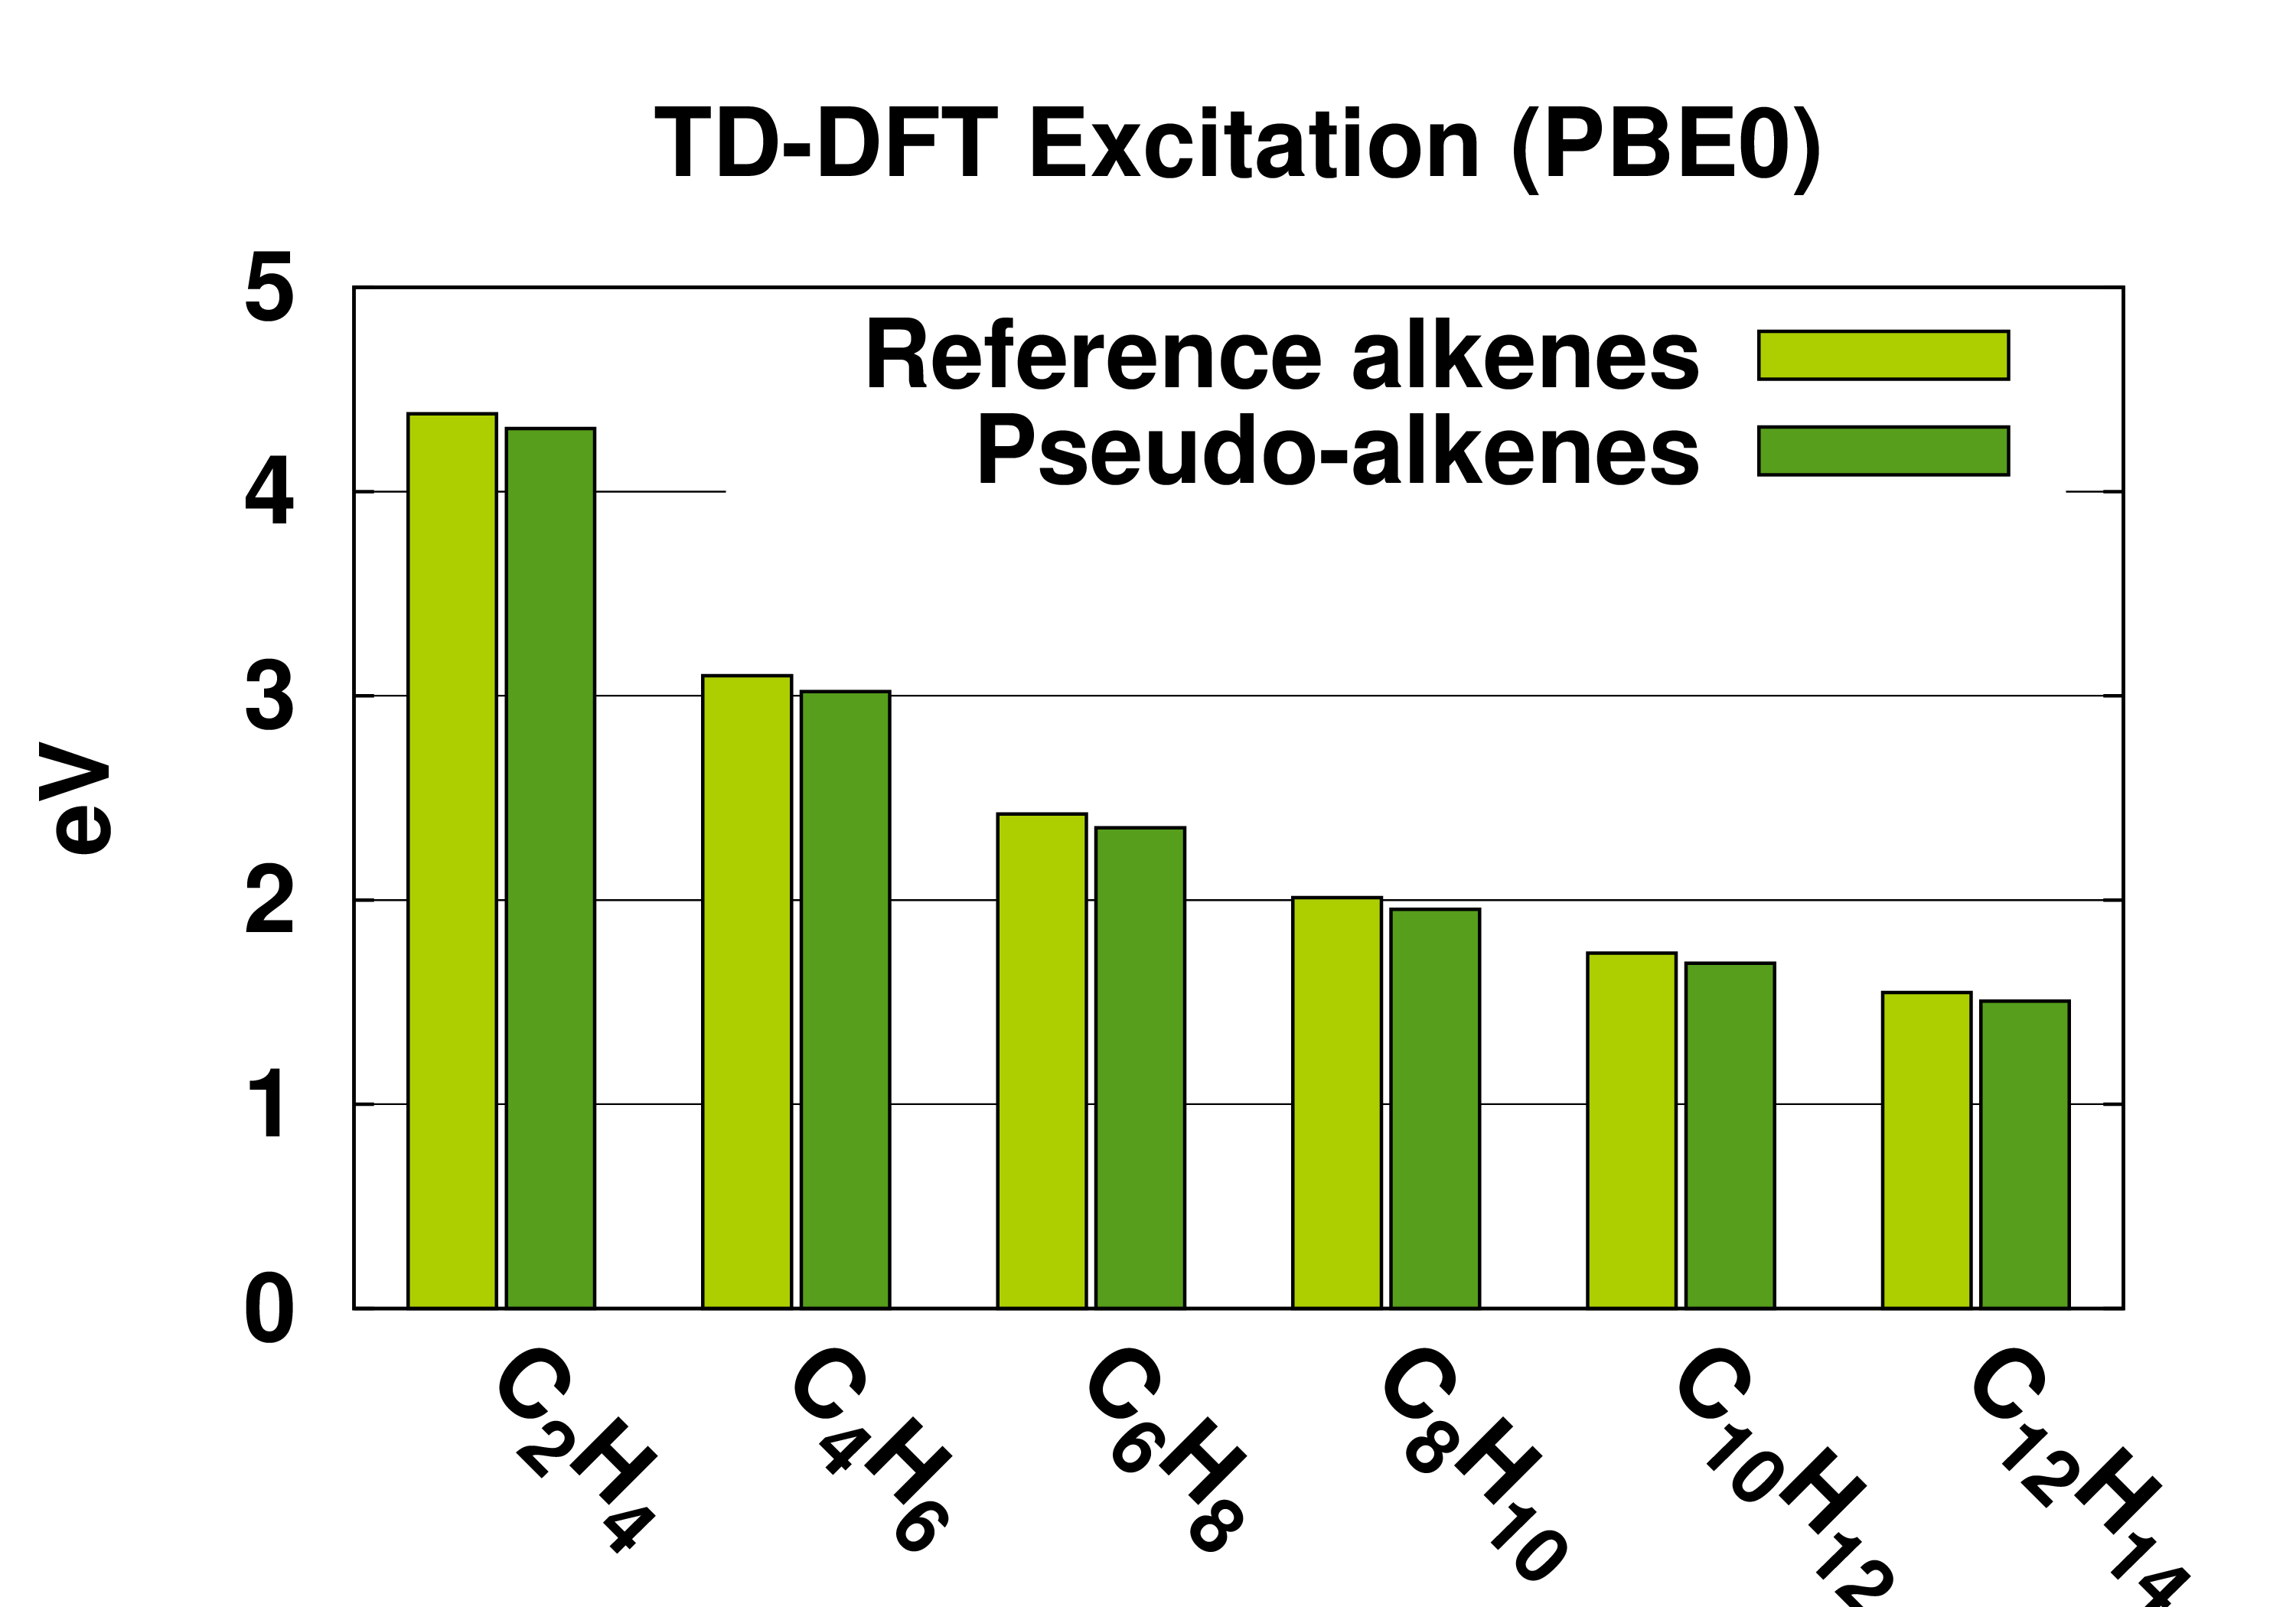
\includegraphics[width=8cm]{short_pbe0_tddft}
\end{center}
\caption{Comparison of pseudo-alkenes with previous (Drujon and Carissan, JCC 2013 (34) 49-59) and current potentials using TD-DFT excitation energies.}
\label{fig:alkenes_tddft}
\end{figure}
Figure \ref{fig:alkenes_tddft} shows the excitation energy of the first triplet $\pi$ excited state
for the six short polyenes studied in the article.
These excitation energies are obtained at the same level of theory both in the previous
version of our work (Drujon and Carissan, JCC 2013 (34) 49-59) and the current work.
As can be seen there is no degradation of the agreement between reference and pseudo-calculations.
The main difference between both these pseudo-systems lies in the fact that in 2013, the pseudo-potentials
had to be placed exactly at the center of the C-C bond whereas in the current work, pseudo-potentials
are placed at a position relative to the center of the pseudo system and do not involve
the C-C distance (the bond direction is still used).

\section*{Full Excited states analysis: singlet and triplet and RPA vs CIS}
As can be seen from figures \ref{fig:cnhn_uv_rpas}, \ref{fig:cnhn_uv_rpat},
\ref{fig:cnhn_uv_ciss} and \ref{fig:cnhn_uv_cist}, Random Phase Approximation (RPA)
and Configuration Interaction Singles (CIS) lead to very similar spectra.
Yet, RPA leads to a better agreement for the calculated intensities.
However, it is worth noting that the decision to use or not the Tamm Dancoff approximation
does not affect the overall good agreement between reference and pseudo-potential.

\section*{Triplet Instability}
The correct treatment of electronic correlation is essential to recover the physics of the ground
and excited states of all-trans-polyenes.\cite{paldus_bond_1983, houk_polyacene_2001, colvin_energies_1998, castano_instabilities_1982, ukrainsky_electronic_1972, sokolov_time-dependent_2017, nakayama_theoretical_1998}

\begin{figure}
\begin{center}
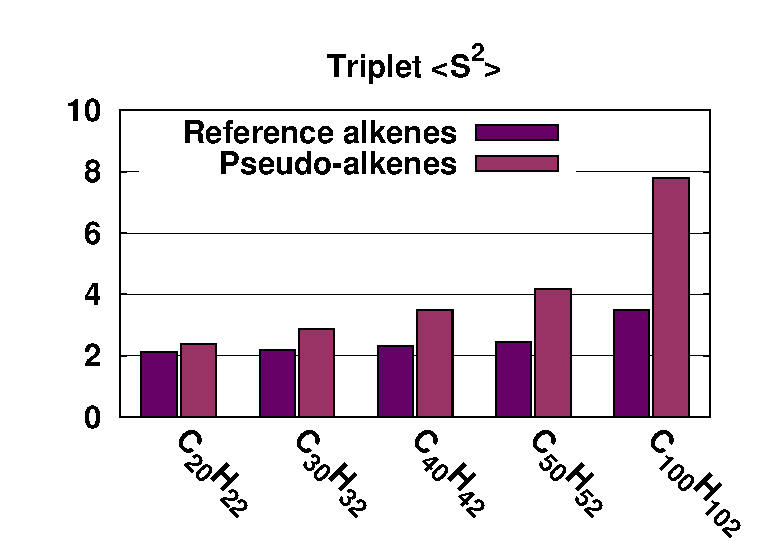
\includegraphics[width=8cm]{long_pbe0_s2}
\end{center}
\caption{Comparison of $S^2$ expectation values obtained for the calculation
of the first $\pi^*$ triplet configuration in a Hartree Fock formalism, for reference
and pseudo-systems.}
\label{fig:ssquare}
\end{figure}

\begin{figure}
\begin{center}
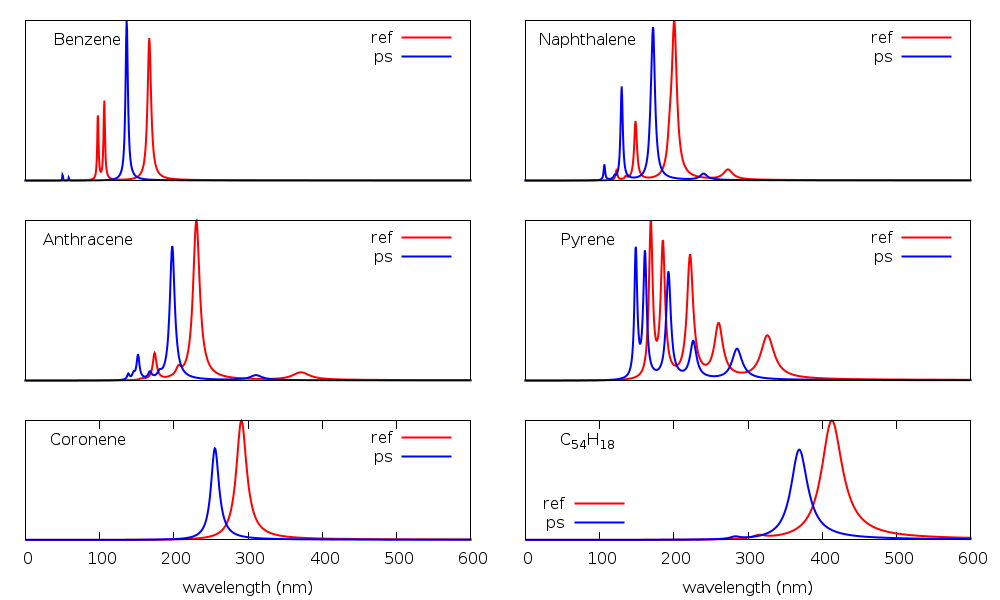
\includegraphics[width=16cm]{grand_rpas}
\end{center}
\vspace{0.25in}
\hspace*{3in}
\caption{Comparison of the absorption spectra for the 20 first singlet excitations obtained with
pseudo-potentials (ps) and all-electron (ref) calculations (def2-SV(P)/TD-PBE0) within the RPA
framework.
Unlike in the main text, the singlet spectra were not shifted by a 0.91 factor.}
\label{fig:cnhn_uv_rpas}
\end{figure}


\begin{figure}
\begin{center}
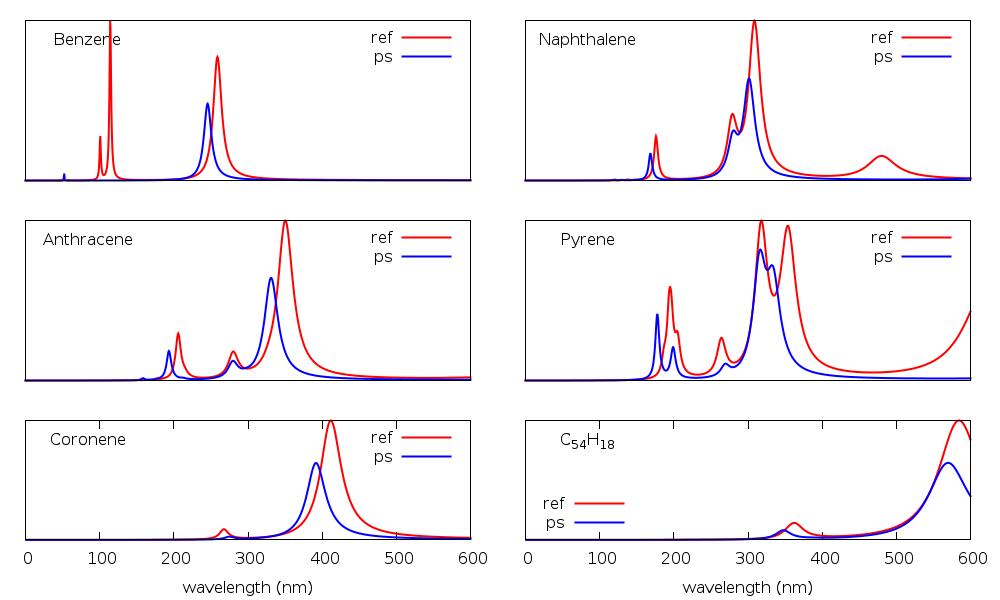
\includegraphics[width=16cm]{grand_rpat}
\end{center}
\vspace{0.25in}
\hspace*{3in}
\caption{Comparison of the absorption spectra for the 20 first triplet excitations obtained with
pseudo-potentials (ps) and all-electron (ref) calculations (def2-SV(P)/TD-PBE0) within the RPA
framework.}
\label{fig:cnhn_uv_rpat}
\end{figure}

\begin{figure}
\begin{center}
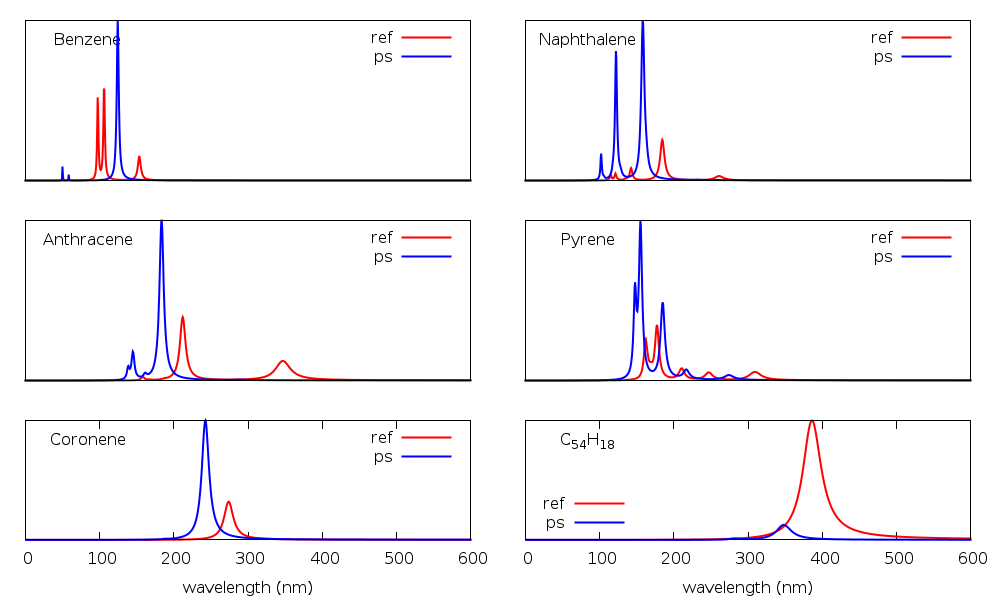
\includegraphics[width=16cm]{grand_ciss}
\end{center}
\vspace{0.25in}
\hspace*{3in}
\caption{Comparison of the absorption spectra for the 20 first singlet excitations obtained with
pseudo-potentials (ps) and all-electron (ref) calculations (def2-SV(P)/TD-PBE0) within the CIS
framework.}
\label{fig:cnhn_uv_cist}
\end{figure}

\begin{figure}
\begin{center}
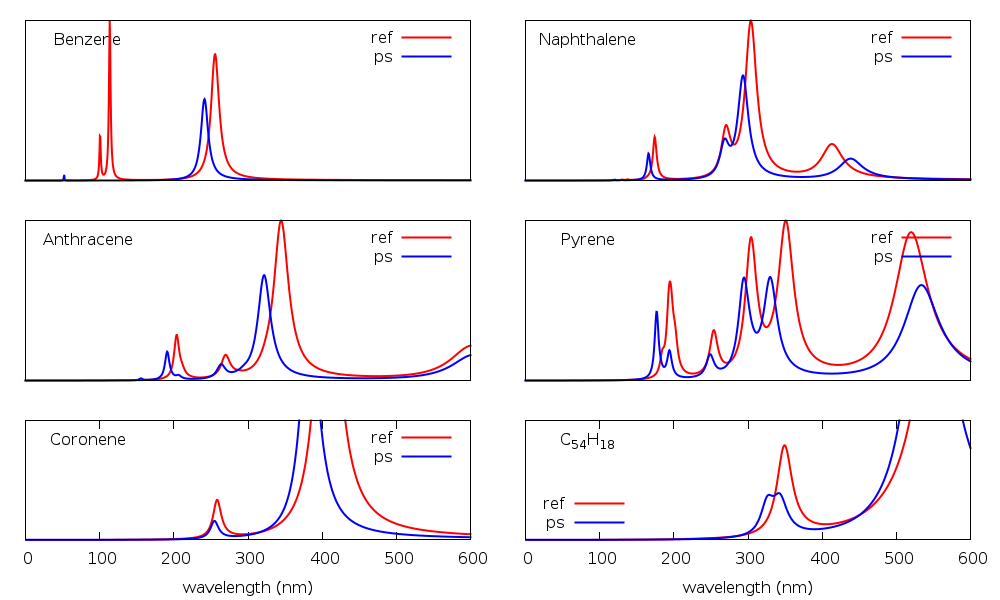
\includegraphics[width=11cm]{grand_cist}
\end{center}
\vspace{0.25in}
\hspace*{3in}
\caption{Comparison of the absorption spectra for the 20 first triplet excitations obtained with
pseudo-potentials (ps) and all-electron (ref) calculations (def2-SV(P)/TD-PBE0) within the CIS
framework.}
\label{fig:cnhn_uv_ciss}
\end{figure}

\clearpage
\section*{B3-LYP Calculations}

Here we report calculations with the B3LYP functional on the spectra of small rings and helicenes.

\begin{figure}[b]
\begin{center}
\includegraphics[width=11cm]{b3_rings_rpas}
\end{center}
%\vspace{0.25in}
\hspace*{3in}
\caption{Comparison of the absorption spectra for the 20 first singlet excitations obtained with
pseudo-potentials (ps) and all-electron (ref) calculations (def2-SV(P)/TD-B3LYP) within the RPA
framework. The wavelength is shifted by a factor of 1.15.}
\label{fig:cnhn_uv_rpas_b3lyp}
\end{figure}

\begin{figure}
\begin{center}
\includegraphics[angle=-90,width=16cm]{b3lyp_grand_rpas}
\end{center}
\vspace{0.25in}
\hspace*{3in}
\caption{Comparison of the absorption spectra of the 20 first singlet excitations for a series of helicene molecules obtained with pseudo-potentials (ps) and all-electron (ref) calculations (def2-SV(P)/TD-B3LYP) within the RPA
framework. The pseudo-molecule wavelength has been corrected by a 32nm shift.}
\label{fig:helicene_spectra_b3lyp}
\end{figure}

\section*{Example Turbomole Input: Benzene}

Below are included example coord, control and basis files for the running of a Turbomole Hartree-Fock calculation for benzene using our pseudo-potential setup.

\subsection*{Coordinate File}

\begin{verbatim}
$coord
   -1.31298477814784     -2.27380782895095      0.00000000000000      c
    1.31271887734650     -2.27406756797785      0.00000000000000      c
    2.62572250864618     -0.00015699191647      0.00000000000000      c
    1.31296575771871      2.27390545849672      0.00000000000000      c
   -1.31275152697941      2.27391013306058      0.00000000000000      c
   -2.62567056810716      0.00004443038124      0.00000000000000      c
   -1.56296714967000     -1.84078494973000     -0.25000000000000      h
   -1.56296714967000     -1.84078494973000      0.25000000000000      h
   -0.81298477856200     -2.27382818432000     -0.25000000000000      h
   -0.81298477856200     -2.27382818432000      0.25000000000000      h
   -1.56300240621000     -2.70681035280000     -0.25000000000000      h
   -1.56300240621000     -2.70681035280000      0.25000000000000      h
    0.81271887979300     -2.27401810714000     -0.25000000000000      h
    0.81271887979300     -2.27401810714000      0.25000000000000      h
    1.56276171047000     -1.84107959863000     -0.25000000000000      h
    1.56276171047000     -1.84107959863000      0.25000000000000      h
    1.56267604178000     -2.70710499817000     -0.25000000000000      h
    1.56267604178000     -2.70710499817000      0.25000000000000      h
    2.37569955168000     -0.43315643878900     -0.25000000000000      h
    2.37569955168000     -0.43315643878900      0.25000000000000      h
    2.37574546631000      0.43286896377800     -0.25000000000000      h
    2.37574546631000      0.43286896377800      0.25000000000000      h
    3.12572250794000     -0.00018350073873     -0.25000000000000      h
    3.12572250794000     -0.00018350073873      0.25000000000000      h
    0.81296575772000      2.27390634865000      0.25000000000000      h
    0.81296575772000      2.27390634865000     -0.25000000000000      h
    1.56296498683000      1.84089231153000      0.25000000000000      h
    1.56296498683000      1.84089231153000     -0.25000000000000      h
    1.56296652861000      2.70691771531000      0.25000000000000      h
    1.56296652861000      2.70691771531000     -0.25000000000000      h
   -1.56276610383000      1.84090584745000      0.25000000000000      h
   -1.56276610383000      1.84090584745000     -0.25000000000000      h
   -0.81275152726300      2.27389330100000      0.25000000000000      h
   -0.81275152726300      2.27389330100000     -0.25000000000000      h
   -1.56273694984000      2.70693125074000      0.25000000000000      h
   -1.56273694984000      2.70693125074000     -0.25000000000000      h
   -2.37568819658000     -0.43297844883900      0.25000000000000      h
   -2.37568819658000     -0.43297844883900     -0.25000000000000      h
   -2.37565294004000      0.43304695422800      0.25000000000000      h
   -2.37565294004000      0.43304695422800     -0.25000000000000      h
   -3.12567056769000      0.00006478575459      0.25000000000000      h
   -3.12567056769000      0.00006478575459     -0.25000000000000      h
$end

\end{verbatim}
\subsection*{Control File}

\begin{verbatim}
$title
$operating system unix
$symmetry cs
$user-defined bonds    file=coord
$coord    file=coord
$optimize
 internal   off
 redundant  off
 cartesian  on
 global     off
 basis      off
$atoms
c  1-6                               \
   basis =c def-SV(P)                \
   ecp   =c ecp-p
h  7-42                              \
   basis =none                       \ 
   ecp   =h ecp-s 
$basis    file=basis 
$ecp    file=basis 
$rundimensions 
   dim(fock,dens)=4221 
   natoms=42 
   nshell=36 
   nbf(CAO)=90 
   dim(trafo[SAO<-->AO/CAO])=102 
   nbf(AO)=84 
$scfiterlimit       30 
$scfconv        7 
$thize     0.10000000E-04 
$thime        5 
$scfdamp   start=1.000  step=0.050  min=0.100 
$scfdump 
$scfintunit 
 unit=30       size=0        file=twoint 
$scfdiis 
$maxcor    500 MiB  per_core 
$scforbitalshift  closedshell=.4 
$drvopt 
   cartesian  on 
   basis      off 
   global     off 
   hessian    on 
   dipole     on 
   nuclear polarizability 
$interconversion  off 
   qconv=1.d-7 
   maxiter=25 
$coordinateupdate 
   dqmax=0.3 
   interpolate  on 
   statistics    5 
$forceupdate 
   ahlrichs numgeo=0  mingeo=3 maxgeo=4 modus=<g|dq> dynamic fail=0.3 
   threig=0.005  reseig=0.005  thrbig=3.0  scale=1.00  damping=0.0 
$forceinit on 
   diag=default 
$energy    file=energy 
$grad    file=gradient 
$forceapprox    file=forceapprox 
$last step     define 
$scfmo none file=mos 
$closed shells 
 a" 1-3 (2) 
$end 

\end{verbatim}

\subsection*{Control File}

\begin{verbatim}
$basis
*
c def-SV(P)
# c     (7s4p1d) / [3s2p1d]     {511/31/1}
*
   5  s
  1238.4016938      0.54568832082E-02
  186.29004992      0.40638409211E-01
  42.251176346      0.18025593888
  11.676557932      0.46315121755
  3.5930506482      0.44087173314
   1  s
 0.40245147363       1.0000000000
   1  s
 0.13090182668       1.0000000000
   3  p
  9.4680970621      0.38387871728E-01
  2.0103545142      0.21117025112
 0.54771004707      0.51328172114
   1  p
 0.15268613795       1.0000000000
   1  d
 0.80000000000       1.0000000000
*
$ecp
*
c ecp-p
*
  ncore =     5           lmax =     3
#        coefficient   r^n          exponent
f
           0.0000000    2           1.0000000
s-f
           0.0000000    1           0.0000000
p-f
          -3.9096200    1           0.6244619
d-f
           0.0000000    1           0.0000000
*
h ecp-s
*
  ncore =     1           lmax =     3
#        coefficient   r^n          exponent
f
           0.0000000    2           1.0000000
s-f
           1.5000000    1           0.5000000
p-f
           0.0000000    1           0.0000000
d-f
           0.0000000    1           0.0000000
*
$end

\end{verbatim}

\clearpage

\bibliography{biblio_pseudo_alex}
\end{document}
